\section{Пример: деревья классификации}
В качестве примера, который демонстрирует пользу кросс-валидации, приведем современную статистическую процедуру, которая называется <<деревья классификации>>. В эксперименте, разработанном для получения информации о причинах возникновения язв двенадцатиперстной кишки, каждой из 745 крыс вводили один из 56 модельных алкилнуклеофилов. Позднее у каждой крысы было проведено вскрытие на предмет развития язвы двенадцатиперстной кишки, и результат был классифицирован как 1, 2 или 3 в порядке возрастания степени тяжести. Было 535 результатов первого класса, 90 --- второго класса и 120 результатов третьего класса. Было измерено шестьдесят семь характеристик этих соединений, и цель анализа состояла в том, чтобы установить, какие из характеристик были связаны с развитием язв двенадцатиперстной кишки.
\begin{figure}[h]
\center{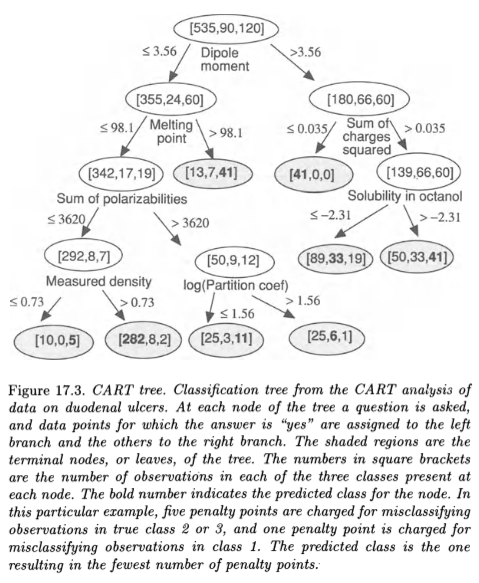
\includegraphics[width=0.8 \linewidth]{17/f17.5.1.png}}
\end{figure}

Рассмотри довольно популярный, но вычислительно затратный алгоритм CART (для деревьев классификации и регрессии) Бреймана, Фридмана, Олшена и Стоуна (1984). Дерево классификации для наших данных, найденное с помощью алгоритма CART показано на рисунке 17.3.

В каждом узле дерева задается <<да-нет>> вопрос, и те данные, для которых дан ответ <<да>>, присваиваются левой ветви, а остальные правой. Листья дерева, показанного на рис. 17.3, называются <<конечными узлами>>. На основе ответов на вопросы каждое наблюдение присваивается одному из конечных узлов. Например, крыса, с дипольным моментом $\leq 3.56$ и точкой плавления $>98.1$, попадает в левый, а затем конечный вправый узел, обозначенный «[13, 7, 41]». 
Три числа, которые изображены под каждым конечным узлом, указывают на количество наблюдений в каждом классе в этом узле, например, для конечного узла с числами «[13, 7, 41]» верно, что в этом конечном узле имеется 13 наблюдений класса 1, 7 наблюдений  класса 2 и 41 наблюдение из класса 2.

Прежде чем обсуждать, как именно это дерево было построено с помощью алгоритма CART, давайте посмотрим, как оно используется для классификации. Каждому конечному узлу назначается класс (1,2 или 3). Самый очевидный способ назначить классы конечным узлам --- это использовать правило большинства и назначить узлу тот класс, который является в нём наиболее многочисленным. Используя правило большинства, узел «[13,7,41]» будет отнесен к классу 3, а все остальные конечные узлы будут отнесены к классу 1. В этом исследовании было решено, что будет в пять раз хуже если мы неправильно классифицируем животное, у которого была тяжелая или умеренная язва, нежели если мы ошибемся с классификацией животного с легкой степенью язвы. Следовательно, если наблюдения из класса 2 и 3 будут классифицированы неверно, то будет начислено пять штрафных баллов, в случае же когда неверно классифицируются наблюдения из класса 1 начисляется один штрафной балл. Прогнозируемый класс --- это тот класс, который дает наименьшее количество штрафных баллов. На рисунке 17.3 на каждом конечном узле жирным шрифтом выделен спрогнозированный класс, например, для узла в левом нижнем углу --- «[10,0,5]» жирным шрифтом выделена цифра 5, следовательно, узел соотносится с классом 3.


Можем сделать следующие выводы по поводу дерева. Верхний («корневой») узел раскололся по дипольному моменту. Высокий дипольный момент указывает на наличие электроотрицательных групп. Происходит разделение на классы 1 и 2: отношение класса 2 к классу 1 в правом разветвлении равно 66/180, что более  чем в 5 раз больше, чем соотношение этих классов в левом разветвлении, равное 24/355. Однако наблюдения класса 3 делятся поровну, по 60 на каждой стороне разветвления. Если при этом сумма квадратов атомных зарядов мала, то CART определяет, что все наблюдения относятся к классу 1. Следовательно, ионизация является основным определяющим фактором биологического действия для наблюдений с высокими дипольными моментами. Двигаясь дальше вниз по правой части дерева, растворимость в октаноле (частично) отделяет класс 3 от класса 2. Высокая растворимость октанола, вероятно, отражает способность проникать через мембраны и проникать в центральную нервную систему. 

На левой стороне корневого узла соединения с низким дипольным моментом и высокой температурой плавления оказались отнесены классу 3. Соединения в этом конечном узле связаны с цистеамином. Наблюдения с низкими температурами плавления и высокой поляризуемостью, то есть все тиолы в этом исследовании, были классифицированы как класс 2 или 3. Химические вещества с низкой поляризуемостью и высокой плотностью относятся к классу 1. Эти химические вещества имеют высокую молекулярную массу и объем, а также этот конечный узел содержит наибольшее количество наблюдений. На стороне разветвления с низкой плотностью все амины с короткой цепью.

В терминологии, упомянутой ранее, набор данных из 745 наблюдений называется обучающей выборкой. Легко вычислить частоту ошибочной классификации для каждого класса, если применить к обучающей выборке дерево, показанное на рис. 17.3. Если посмотреть на конечные узлы, которые предсказывают классы 2 или 3, количество ошибок для класса 1 составляет $13 + 89 + 50 + 10 + 25 + 25 = 212$, поэтому видимый процент ошибочной классификации для класса 1 составляет $212/535 = 39.6 \%$. Аналогичным образом, видимые коэффициенты ошибочной классификации для классов 2 и 3 составляют $56.7 \%$ и $18,3\%$. «Видимый» является здесь важным уточнением, поскольку частота ошибочной классификации для обучающей выборке может быть сильно смещена в сторону понижения по той же причине, по которой квадрат остаточной ошибки слишком оптимистичен для регрессии.

Как CART строит дерево, которое изображено на рис. 17.3? CART - это полностью автоматическая процедура, которая выбирает переменные и значения, по которым  данные лучше всего делятся на классы. Например, «дипольный момент$ \ \leq 3.56$» --- было выбрано лучшим правилом для разделения данных на классы. CART выбрал как переменную по которой происходит раздление --- «дипольный момент», так и граничное значение, которое равно $3.56$. После того как было выбрано первое правило для разделения, новые правила разделения выбираются для каждой из двух полученных после первого разделения групп, и этот процесс повторяется. 

Вместо того, чтобы остановить алогритм, когда дерево достигает некоторого разумного размера, CART использует более эффективный подход: создается большое дерево, которое затем обрезается снизу. Это более эффективный подход для обнаружения взаимосвязей, в которых участвует несколько переменных.

Возникает важный вопрос: какого размера должно быть дерево? Если мы построили бы очень большое дерево у которого было бы только одно наблюдение в каждом конечном узле, то видимая вероятность ошибочной классификации составила бы $0 \%$. Однако, это дерево не справится с предсказанием результатов для новой выборки. Причина в том, что дерево будет ориентировано на обучающую выборку --- это «переобучение».

Дерево наилучшего размера --- это такое дерево, которое дает наименьшую ошибку классификации на новых данных. Таким образом, если бы у нас был второй набор данных (тестовая выборка), мы могли бы применить к нему деревья разных размеров, а затем выбрать то дерево, у которого самое маленько количество ошибок классификации.

В большинстве ситуаций у нас нет дополнительных данных, поэтом воспользуемся кросс-валидацией. Leave-one-out кросс-валидация не подойдет для нашего случая, потому что результирующие деревья не будут достаточно отличаться от исходного дерева. Опыт показывает, что гораздо лучше разделить данные на $10$ групп равного размера, построить дерево для $90 \%$ данных, а затем оценить уровень ошибочной классификации на оставшихся $10 \%$ данных. Это делается по очереди для каждой из 10 групп, и общий коэффициент ошибочной классификации вычисляется за 10 прогонов. Лучшим размером дерева считается тот размер дерева, который дает наименьшую вероятность ошибочной классификации. Этот размер будет использоваться для построения окончательного дерева на всех данных. Важнейшей особенностью кросс-валидации является разделение данных для построения и оценки деревьев: каждая десятая часть данных выступает в качестве тестовой выборки для остальных девяти частей. 

Кросс-валидация позволяет не только получить оценку для лучшего размера дерева, но также дает реалистичную оценку уровня ошибочной классификации для окончательного дерева. Вычисленные выше видимые ошибки часто оказывются ниже, потому что обучающая выборка используется как для построения, так и для оценки дерева. Для дерева на рис. 17.3 частота ошибочной классификации с проверкой, с помощью кросс-валидации, была примерно на $10 \%$ выше, чем частота видимых ошибок. Уровень ошибки вычесленный с помощью кросс-валидации обеспечивает точную оценку того, насколько эффективно дерево будет классифицировать новую выборку.
